\question \textbf{Lookup table for n-grams}
  
Create a 2-gram lookup table with indices and scores for the sequence q: ATGCAT. 

\medskip 

Score matrix:
\begin{figure}[H]
      \centering
      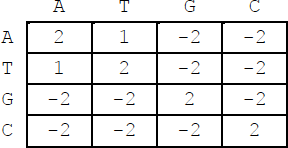
\includegraphics[width=0.25 \textwidth]{fig05/score_scheme_2.png}
\end{figure}

 T: 3 \\

Pre-calculated scores of all segment pairs:
\begin{figure}[H]
      \centering
      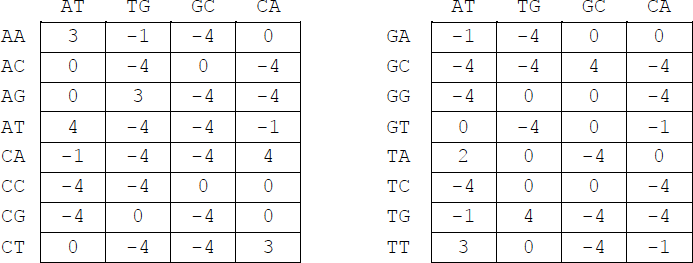
\includegraphics[width=0.65 \textwidth]{fig05/lookup_table_precalculated.png}
\end{figure}

\begin{parts}

%% (a)
  \part Fill the table.

\begin{figure}[H]
      \centering
      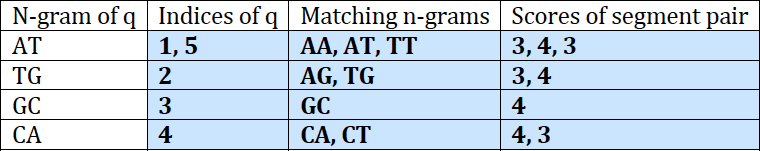
\includegraphics[width=0.65 \textwidth]{fig05/lookup_table_n-gram_solution.png}
\end{figure}

%% (b)
\part Create a lookup table for the matching n-grams with scores and indices.

\begin{figure}[H]
      \centering
      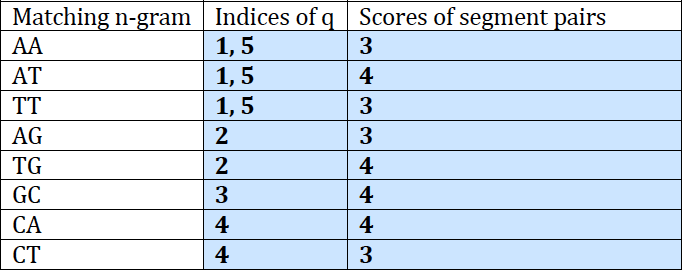
\includegraphics[width=0.6 \textwidth]{fig05/lookup_table_n-gram_final_solution.png}
\end{figure}

\end{parts}